\documentclass[aspectratio=169,10pt]{beamer}

\usepackage[T1]{fontenc}
\usepackage{lmodern}
\usepackage{amsmath,amssymb}
\usepackage{booktabs}
\usepackage{array}
\usepackage{colortbl}
\usepackage{tikz}
\usetikzlibrary{arrows.meta,positioning,shapes.geometric,calc,decorations.pathreplacing}

\definecolor{Navy}{HTML}{17324D}
\definecolor{Blue}{HTML}{2374AB}
\definecolor{Cyan}{HTML}{3AAFA9}
\definecolor{Orange}{HTML}{F28E2B}
\definecolor{Red}{HTML}{D9534F}
\definecolor{Green}{HTML}{3A7D44}
\definecolor{Light}{HTML}{F3F6F8}
\definecolor{Mid}{HTML}{D9E2E8}
\definecolor{Text}{HTML}{23313A}

\usetheme{default}
\setbeamercolor{normal text}{fg=Text,bg=white}
\setbeamercolor{frametitle}{fg=Navy,bg=white}
\setbeamercolor{title}{fg=white}
\setbeamercolor{subtitle}{fg=white}
\setbeamercolor{structure}{fg=Blue}
\setbeamercolor{block title}{fg=white,bg=Navy}
\setbeamercolor{block body}{fg=Text,bg=Light}
\setbeamercolor{alertblock title}{fg=white,bg=Orange}
\setbeamercolor{alertblock body}{fg=Text,bg=Orange!10}
\setbeamertemplate{navigation symbols}{}
\setbeamertemplate{itemize item}{\color{Blue}\small$\blacktriangleright$}
\setbeamertemplate{itemize subitem}{\color{Cyan}\scriptsize$\bullet$}
\setbeamertemplate{footline}{%
  \leavevmode%
  \hbox{%
    \begin{beamercolorbox}[wd=.78\paperwidth,ht=2.7ex,dp=1.2ex,leftskip=1em]{author in head/foot}%
      \color{Navy}\scriptsize Layout Management Progress Meeting
    \end{beamercolorbox}%
    \begin{beamercolorbox}[wd=.22\paperwidth,ht=2.7ex,dp=1.2ex,rightskip=1em plus1fil]{date in head/foot}%
      \color{Navy}\scriptsize\insertframenumber/\inserttotalframenumber
    \end{beamercolorbox}}%
}
\setbeamertemplate{frametitle}{%
  \vspace{0.35em}\insertframetitle\par
  \vspace{-0.35em}\color{Mid}\rule{\textwidth}{0.6pt}
}

\newcommand{\pill}[2]{%
  \tikz[baseline=(n.base)]\node[rounded corners=2pt,fill=#1!14,
  text=#1,inner xsep=5pt,inner ysep=2pt,font=\scriptsize\bfseries](n){#2};}
\newcommand{\metric}[3]{%
  \begin{minipage}[t]{0.29\textwidth}
    \centering{\color{#1}\LARGE\bfseries #2}\\[-1mm]
    {\scriptsize #3}
  \end{minipage}}
\newcommand{\source}[1]{\vfill{\tiny\color{gray}Source: #1}}

\title{Warehouse Slotting and Traffic Optimization}
\subtitle{Progress meeting: approach, algorithms, and current evidence}
\author{Layout Management Project}
\date{5 August 2026}

\begin{document}

% 1
\begin{frame}[plain]
  \begin{tikzpicture}[remember picture,overlay]
    \fill[Navy] (current page.south west) rectangle (current page.north east);
    \fill[Blue] ([xshift=9.9cm]current page.south west)
      -- (current page.south east) -- (current page.north east)
      -- ([xshift=13.1cm]current page.north west) -- cycle;
    \draw[Cyan,line width=2pt] ([xshift=0.9cm,yshift=1.05cm]current page.south west)
      -- ([xshift=6.1cm,yshift=1.05cm]current page.south west);
  \end{tikzpicture}
  \vspace{1.45cm}
  {\usebeamerfont{title}\color{white}\LARGE\bfseries\inserttitle\par}
  \vspace{0.35cm}
  {\color{white!82}\large\insertsubtitle\par}
  \vspace{0.85cm}
  \pill{Cyan}{ABC SLOTTING}\quad
  \pill{Cyan}{AFFINITY}\quad
  \pill{Orange}{TRAFFIC-AWARE}\quad
  \pill{Orange}{GLOBAL OPTIMIZATION}
  \vfill
  {\color{white!75}\small\insertauthor\hfill\insertdate}
  \vspace{0.6cm}
\end{frame}

% 2
\begin{frame}{Progress at a glance}
  \begin{columns}[T,onlytextwidth]
    \column{0.56\textwidth}
    \begin{block}{What is implemented}
      \begin{itemize}
        \item ABC velocity classification and physical profile extraction
        \item Store-day affinity identification and affinity-aware placement
        \item Paper-replication C\&TBSA clustering and shelf assignment
        \item Global, time-bounded CP-SAT placement optimization
      \end{itemize}
    \end{block}
    \column{0.40\textwidth}
    \begin{alertblock}{Meeting focus}
      How the four methods fit together, what each optimizes, and how hard
      warehouse rules remain protected.
    \end{alertblock}
    \vspace{0.2cm}
    \begin{minipage}[t]{0.46\linewidth}
      \centering{\color{Blue}\LARGE\bfseries 1,524}\\[-1mm]
      {\scriptsize SKUs in velocity summary}
    \end{minipage}\hfill
    \begin{minipage}[t]{0.46\linewidth}
      \centering{\color{Green}\LARGE\bfseries 4}\\[-1mm]
      {\scriptsize implemented stages}
    \end{minipage}
  \end{columns}
  \source{Repository implementation and current generated artifacts.}
\end{frame}

% 3
\begin{frame}{C\&TBSA is a direct pipeline}
  \centering
  
\begin{tikzpicture}[
    box/.style={rounded corners=3pt,minimum width=3.35cm,minimum height=1.15cm,
      align=center,font=\small\bfseries,text=white},
    arr/.style={-{Latex[length=2mm]},line width=1.2pt,color=Navy}
  ]
    \node[box,fill=Navy] (data) {Warehouse grid\\SKU physical data\\order history};
    \node[box,fill=Orange,right=10mm of data] (ctbsa)
      {Paper C\&TBSA\\demand + correlation\\NSGA-II clustering};
    \node[box,fill=Green,right=10mm of ctbsa] (layout)
      {Final shelf layout\\+ static traffic\\validation};
    \draw[arr] (data)--(ctbsa);
    \draw[arr] (ctbsa)--(layout);
  \end{tikzpicture}
  \vspace{0.55cm}
  \begin{block}{Not prerequisite stages}
    \centering
    \pill{Blue}{ABC SLOTTING: COMPARISON}\qquad
    \pill{Cyan}{AFFINITY SLOTTING: COMPARISON}\qquad
    \pill{Green}{GLOBAL CP-SAT: SEPARATE MODEL}
  \end{block}
  \vspace{0.25cm}
  \begin{alertblock}{Why a feasibility seed still exists internally}
    It reserves chilled and physical-exception storage and checks hard rules.
    Eligible standard-SKU membership is then discarded and rebuilt by C\&TBSA.
  \end{alertblock}
\end{frame}
% 4
\begin{frame}{Two constraint layers define the feasible C\&TBSA layout}
  \begin{columns}[T,onlytextwidth]
    \column{0.47\textwidth}
    \begin{block}{Paper model: reproduced}
      \[
        \sum_k x_{jk}=1,\qquad
        \sum_j x_{jk}\le Z_k
      \]
      \[
        \sum_j F_jx_{jk}\le W_{\max},\qquad
        x_{jk}\in\{0,1\}
      \]
      \scriptsize
      Every SKU enters one cluster; each cluster fits its storage-location count;
      $W_{\max}$ is at least every cluster's demand.
    \end{block}
    \column{0.49\textwidth}
    \begin{alertblock}{Warehouse safety: added feasibility}
      \begin{itemize}
        \item AMR shelf with one ordinary SKU per location
        \item unique occupied addresses
        \item chilled and ambient separation
        \item inherited attributes and physical capacity
        \item oversize, overweight, multi-slot, or incomplete racks fixed
      \end{itemize}
    \end{alertblock}
  \end{columns}
  \vspace{0.3cm}
  \centering
  
\begin{tikzpicture}[
    card/.style={rounded corners=3pt,draw=Green,fill=Green!10,
      minimum width=11.8cm,minimum height=0.82cm,align=center,font=\scriptsize\bfseries}
  ]
    \node[card] {C\&TBSA searches only assignments satisfying both layers};
  \end{tikzpicture}
  \source{Warehouse rules restrict feasibility; they do not change the paper's two objectives.}
\end{frame}
% 5
\begin{frame}{ABC identification: convert demand into velocity priority}
  \begin{columns}[T,onlytextwidth]
    \column{0.56\textwidth}
    \[
      f_i = \#\{\text{pick lines for SKU }i\},\qquad
      c_k = \frac{\sum_{i=1}^{k}f_{(i)}}{\sum_j f_j}
    \]
    {\scriptsize $i,j$: SKU indices;\quad $k$: position in the sorted list;\quad
    $f_i$: pick frequency;\quad $f_{(i)}$: $i$th-highest frequency;\quad
    $c_k$: cumulative pick share through rank $k$.}

    \begin{enumerate}
      \item Count pick frequency per SKU.
      \item Sort SKUs by descending $f_i$.
      \item Compute cumulative demand share $c_k$.
      \item Assign A through 80\%, B through 95\%, then C.
    \end{enumerate}
    \column{0.40\textwidth}
    
\begin{tikzpicture}[x=0.045cm,y=0.047cm]
      \fill[Blue!85] (0,0) rectangle (80,16);
      \fill[Cyan!80] (80,0) rectangle (95,16);
      \fill[Orange!85] (95,0) rectangle (100,16);
      \node[white,font=\bfseries] at (40,8) {A: 80\%};
      \node[white,font=\bfseries,rotate=90] at (87.5,8) {B: 15\%};
      \node[Text,font=\scriptsize,rotate=90] at (97.5,8) {C: 5\%};
      \draw[->,Navy] (0,-2)--(102,-2);
      \node[font=\scriptsize,anchor=north] at (51,-3) {cumulative pick share};
    \end{tikzpicture}
    \vspace{0.45cm}
    \begin{block}{Why frequency, not quantity?}
      It targets handling events and travel triggers; unit quantity remains a
      separate inventory measure.
    \end{block}
  \end{columns}
\end{frame}

% 6
\begin{frame}{Pure ABC slotting algorithm}
  \centering
  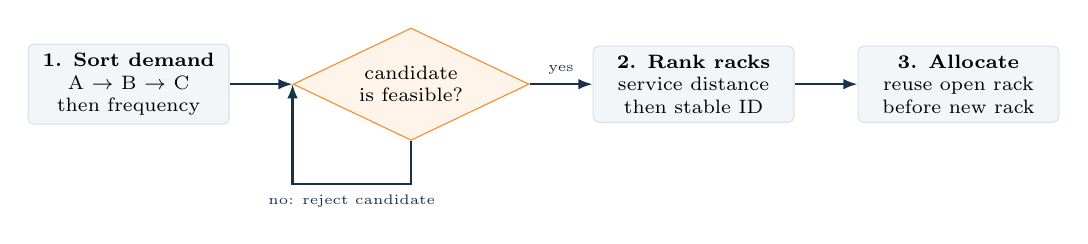
\begin{tikzpicture}[
    node distance=5mm and 8mm,
    proc/.style={rounded corners=2pt,draw=Mid,fill=Light,minimum width=2.55cm,
      minimum height=0.85cm,align=center,font=\scriptsize},
    decision/.style={diamond,aspect=2.1,draw=Orange,fill=Orange!10,
      align=center,font=\scriptsize},
    arr/.style={-{Latex[length=1.8mm]},Navy,thick}
  ]
    \node[proc] (sort) {\textbf{1. Sort demand}\\A $\rightarrow$ B $\rightarrow$ C\\then frequency};
    \node[decision,right=of sort] (fit) {candidate\\is feasible?};
    \node[proc,right=of fit] (rank) {\textbf{2. Rank racks}\\service distance\\then stable ID};
    \node[proc,right=of rank] (alloc) {\textbf{3. Allocate}\\reuse open rack\\before new rack};
    \draw[arr] (sort)--(fit);
    \draw[arr] (fit)--node[above,font=\tiny]{yes}(rank);
    \draw[arr] (rank)--(alloc);
    \draw[arr] (fit.south) |- ++(0,-0.55) -| node[pos=.25,below,font=\tiny]{no: reject candidate} (fit.west);
  \end{tikzpicture}
  \vspace{0.55cm}
  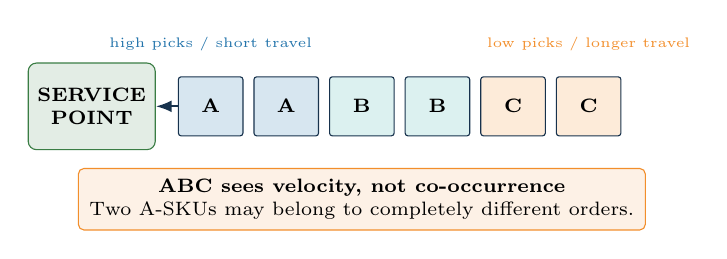
\begin{tikzpicture}[
    rack/.style={draw=Navy,rounded corners=1pt,minimum width=0.82cm,
      minimum height=0.75cm,font=\scriptsize\bfseries},
    arr/.style={-{Latex[length=2mm]},thick,Navy}
  ]
    \node[draw=Green,fill=Green!14,rounded corners=3pt,minimum width=1.6cm,
      minimum height=1.1cm,font=\scriptsize\bfseries,align=center] (ws)
      {SERVICE\\POINT};
    \foreach \x/\lab/\col in {0/A/Blue,1/A/Blue,2/B/Cyan,3/B/Cyan,4/C/Orange,5/C/Orange}{
      \node[rack,fill=\col!18,right=0.28cm of ws,xshift=\x*0.96cm] (r\x) {\lab};
    }
    \draw[arr] (r0.west)--(ws.east);
    \node[above=2mm of r0,font=\tiny,text=Blue] {high picks / short travel};
    \node[above=2mm of r5,font=\tiny,text=Orange] {low picks / longer travel};
    \node[below=4mm of r2,rounded corners=2pt,fill=Orange!12,draw=Orange,
      inner sep=4pt,font=\scriptsize,align=center]
      {\textbf{ABC sees velocity, not co-occurrence}\\
       Two A-SKUs may belong to completely different orders.};
  \end{tikzpicture}
\end{frame}

% 7
\begin{frame}{Affinity identification: find SKUs requested together}
  \begin{columns}[T,onlytextwidth]
    \column{0.55\textwidth}
    One fulfilment group is a \textbf{(Store ID, Date)} pair. Presence is binary:
    \[
      X_{g,i} =
      \begin{cases}
        1,&\text{SKU }i\text{ occurs in group }g\\
        0,&\text{otherwise}
      \end{cases}
    \]
    \[
      N(i,j)=\sum_g X_{g,i}X_{g,j},\qquad
      A(i,j)=\frac{N(i,j)}
      {\sqrt{N(i)N(j)}}
    \]
    {\scriptsize $g$: store-day group;\quad $i,j$: SKUs;\quad
    $N(i,j)$: shared-group count;\quad
    $N(i)=\sum_gX_{g,i}$: groups containing SKU $i$;\quad
    $A(i,j)$: cosine affinity in $[0,1]$.}

    \column{0.41\textwidth}
    \centering
    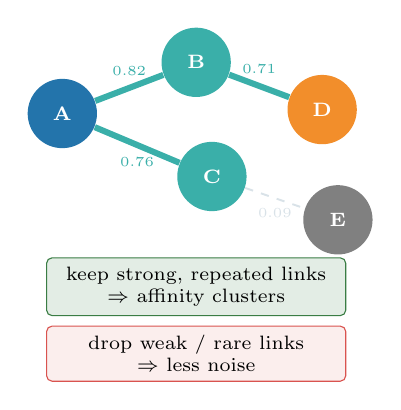
\begin{tikzpicture}[
      sku/.style={circle,minimum size=0.88cm,text=white,font=\scriptsize\bfseries},
      edge/.style={Cyan,line width=2.2pt},
      weak/.style={Mid,line width=0.7pt,dashed}
    ]
      \node[sku,fill=Blue] (a) at (0,1.7) {A};
      \node[sku,fill=Cyan] (b) at (1.7,2.35) {B};
      \node[sku,fill=Cyan] (c) at (1.9,0.9) {C};
      \node[sku,fill=Orange] (d) at (3.3,1.75) {D};
      \node[sku,fill=gray] (e) at (3.5,0.35) {E};
      \draw[edge] (a)--node[above,font=\tiny]{0.82}(b);
      \draw[edge] (a)--node[below,font=\tiny]{0.76}(c);
      \draw[edge] (b)--node[above,font=\tiny]{0.71}(d);
      \draw[weak] (c)--node[below,font=\tiny]{0.09}(e);
      \node[rounded corners=2pt,fill=Green!14,draw=Green,align=center,
        font=\scriptsize,minimum width=3.8cm] at (1.7,-0.5)
        {keep strong, repeated links\\$\Rightarrow$ affinity clusters};
      \node[rounded corners=2pt,fill=Red!10,draw=Red,align=center,
        font=\scriptsize,minimum width=3.8cm] at (1.7,-1.35)
        {drop weak / rare links\\$\Rightarrow$ less noise};
    \end{tikzpicture}
  \end{columns}
\end{frame}

% 8
\begin{frame}{Affinity identification workflow}
  \centering
  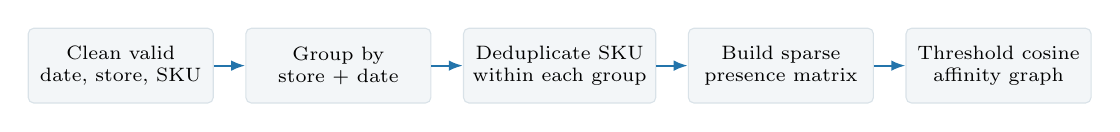
\begin{tikzpicture}[
    node distance=4mm,
    box/.style={rounded corners=2pt,draw=Mid,fill=Light,minimum width=2.35cm,
      minimum height=0.95cm,align=center,font=\scriptsize},
    arr/.style={-{Latex[length=1.8mm]},Blue,thick}
  ]
    \node[box] (clean) {Clean valid\\date, store, SKU};
    \node[box,right=of clean] (group) {Group by\\store + date};
    \node[box,right=of group] (binary) {Deduplicate SKU\\within each group};
    \node[box,right=of binary] (matrix) {Build sparse\\presence matrix};
    \node[box,right=of matrix] (graph) {Threshold cosine\\affinity graph};
    \draw[arr] (clean)--(group);
    \draw[arr] (group)--(binary);
    \draw[arr] (binary)--(matrix);
    \draw[arr] (matrix)--(graph);
  \end{tikzpicture}
  \vspace{0.7cm}
  \begin{columns}[T,onlytextwidth]
    \column{0.47\textwidth}
    \centering
    {\scriptsize\bfseries Raw lines: duplicates retained for $F(i,s)$}\\[1mm]
    \begin{tabular}{c|ccc}
      & A & B & C\\\hline
      Store 1, Day 1 & \cellcolor{Blue!30}2 & \cellcolor{Blue!18}1 & 0\\
      Store 1, Day 2 & 0 & \cellcolor{Blue!18}1 & \cellcolor{Blue!18}1\\
    \end{tabular}
    \column{0.49\textwidth}
    \centering
    {\scriptsize\bfseries Binary presence used for affinity}\\[1mm]
    \begin{tabular}{c|ccc}
      & A & B & C\\\hline
      $g_1$ & \cellcolor{Cyan!30}1 & \cellcolor{Cyan!30}1 & 0\\
      $g_2$ & 0 & \cellcolor{Cyan!30}1 & \cellcolor{Cyan!30}1\\
    \end{tabular}\\[1mm]
    {\tiny Duplicate A lines become one presence signal.}
  \end{columns}
  \source{Affinity analysis module and slotting support utilities.}
\end{frame}

% 9
\begin{frame}{ABC + affinity slotting: blend two useful signals}
  \begin{columns}[T,onlytextwidth]
    \column{0.59\textwidth}
    Candidate ordering uses:
    \[
      J_i =
      (1-w)\,\underbrace{C_i}_{\text{ABC cost}}
      +w\,\underbrace{\left(1-\frac{O_i}{O_{\max}}\right)}_{\text{affinity cost}},
      \qquad 0\leq w\leq1
    \]
    {\scriptsize $J_i$: selection cost;\quad $C_i$: normalized ABC-class cost;\quad
    $w$: affinity weight;\quad $O_i$: candidate-to-cluster group overlap;\quad
    $O_{\max}$: largest overlap among remaining candidates.}

    \begin{enumerate}
      \item Start a rack cluster with the strongest demand signal.
      \item Select the feasible SKU with minimum blended cost.
      \item Update the cluster mask; reset when rack capacity is reached.
    \end{enumerate}
    \column{0.37\textwidth}
    \centering
    {\scriptsize\bfseries Affinity-weight control}\\[1mm]
    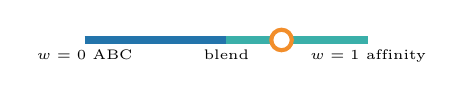
\begin{tikzpicture}
      \draw[line width=3pt,Blue] (0,0)--(1.8,0);
      \draw[line width=3pt,Cyan] (1.8,0)--(3.6,0);
      \draw[fill=white,draw=Orange,line width=1.5pt] (2.5,0) circle (0.13);
      \node[below,font=\tiny] at (0,0) {$w=0$ ABC};
      \node[below,font=\tiny] at (1.8,0) {blend};
      \node[below,font=\tiny] at (3.6,0) {$w=1$ affinity};
    \end{tikzpicture}
    \vspace{0.45cm}

    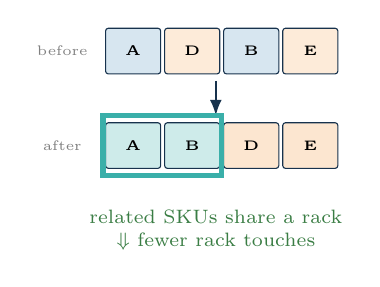
\begin{tikzpicture}[
      bin/.style={draw=Navy,rounded corners=1pt,minimum width=0.7cm,
        minimum height=0.58cm,font=\tiny\bfseries}
    ]
      \node[font=\tiny,text=gray] at (-0.3,1.0) {before};
      \node[bin,fill=Blue!18] at (0.6,1.0) {A};
      \node[bin,fill=Orange!18] at (1.35,1.0) {D};
      \node[bin,fill=Blue!18] at (2.1,1.0) {B};
      \node[bin,fill=Orange!18] at (2.85,1.0) {E};
      \draw[-{Latex[length=2mm]},thick,Navy] (1.65,0.62)--(1.65,0.18);
      \node[font=\tiny,text=gray] at (-0.3,-0.2) {after};
      \node[bin,fill=Cyan!25] at (0.6,-0.2) {A};
      \node[bin,fill=Cyan!25] at (1.35,-0.2) {B};
      \node[bin,fill=Orange!22] at (2.1,-0.2) {D};
      \node[bin,fill=Orange!22] at (2.85,-0.2) {E};
      \draw[Cyan,line width=2pt] (0.22,-0.58) rectangle (1.72,0.18);
      \node[below=4mm,font=\scriptsize,align=center,text=Green] at (1.65,-0.5)
        {related SKUs share a rack\\$\Downarrow$ fewer rack touches};
    \end{tikzpicture}
  \end{columns}
\end{frame}

% 10
\begin{frame}{Notation reference: ABC and affinity}
  \small
  \begin{tabular}{@{}p{0.16\textwidth}p{0.76\textwidth}@{}}
    \toprule
    \textbf{Symbol} & \textbf{Meaning}\\
    \midrule
    $i,j$ & SKU indices; $(i)$ denotes position after descending-frequency sorting.\\
    $k$ & Final rank included in a cumulative ABC calculation.\\
    $s,g$ & Store index $s$; fulfilment-group index $g=(\text{Store ID},\text{Date})$.\\
    $f_i,c_k$ & Pick frequency for SKU $i$; cumulative pick share through rank $k$.\\
    $F(i,s)$ & Direct line-order frequency between SKU $i$ and store $s$.\\
    $X_{g,i}$ & Binary indicator: 1 when group $g$ contains SKU $i$, otherwise 0.\\
    $N(i),N(i,j)$ & Groups containing $i$; groups containing both $i$ and $j$.\\
    $A(i,j)$ & Cosine affinity between SKUs $i$ and $j$, from 0 to 1.\\
    $J_i,C_i$ & Blended selection cost; normalized ABC-class component.\\
    $w,O_i,O_{\max}$ & Affinity weight; candidate overlap; maximum candidate overlap.\\
    $\mathcal{F},p$ & Set of hard-rule-feasible placements; one candidate placement.\\
    \bottomrule
  \end{tabular}
\end{frame}

% 11
\begin{frame}{Why a good slotting layout can still create traffic}
  \begin{columns}[T,onlytextwidth]
    \column{0.56\textwidth}
    \centering
    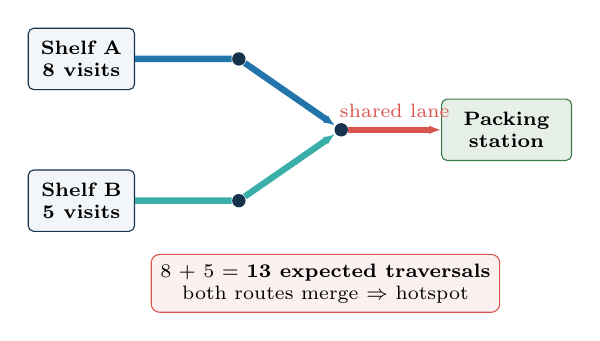
\begin{tikzpicture}[
      loc/.style={rounded corners=2pt,draw=Navy,fill=Light,minimum width=1.35cm,
        minimum height=0.78cm,font=\scriptsize\bfseries,align=center},
      junction/.style={circle,fill=Navy,minimum size=0.17cm,inner sep=0pt},
      route/.style={-{Latex[length=1.5mm]},line width=2.3pt}
    ]
      \node[loc] (u1) at (0,2.7) {Shelf A\\8 visits};
      \node[loc] (u2) at (0,0.9) {Shelf B\\5 visits};
      \node[junction] (j1) at (2.0,2.7) {};
      \node[junction] (j2) at (2.0,0.9) {};
      \node[junction] (merge) at (3.3,1.8) {};
      \node[loc,draw=Green,fill=Green!12,minimum width=1.65cm] (endpoint)
        at (5.4,1.8) {Packing\\station};
      \draw[route,Blue] (u1)--(j1)--(merge);
      \draw[route,Cyan] (u2)--(j2)--(merge);
      \draw[route,Red] (merge)--node[above,font=\scriptsize,text=Red]
        {shared lane}(endpoint);
      \node[rounded corners=3pt,draw=Red,fill=Red!8,font=\scriptsize,
        align=center,minimum width=4.2cm] at (3.1,-0.15)
        {8 + 5 = \textbf{13 expected traversals}\\
         both routes merge $\Rightarrow$ hotspot};
    \end{tikzpicture}
    \column{0.40\textwidth}
    \begin{block}{How load is calculated}
      \begin{enumerate}
        \item Group orders by store and date.
        \item Count visits to each complete shelf or tote.
        \item Route every visit to a service endpoint.
        \item Add the visits on every shared lane.
      \end{enumerate}
    \end{block}
    \begin{alertblock}{Optimization question}
      Can reassignment distribute expected demand while preserving affinity and
      physical feasibility?
    \end{alertblock}
  \end{columns}
  \source{AMR counts one shelf visit per task; ASRS counts each required physical retrieval.}
\end{frame}

\section{Traffic-aware C\&TBSA reproduction}

\begin{frame}{Updated traffic-aware workflow: Affinity first, then C\&TBSA}
  \centering
  
\begin{tikzpicture}[
    box/.style={rounded corners=3pt,minimum width=2.42cm,minimum height=1.02cm,
      align=center,font=\scriptsize\bfseries,text=white},
    arr/.style={-{Latex[length=2mm]},thick,Navy}
  ]
    \node[box,fill=Navy] (input) {Grid JSON\\SKU physical CSV\\order workbook};
    \node[box,fill=Blue,right=3mm of input] (seed) {ABC + Affinity\\baseline};
    \node[box,fill=Orange,right=3mm of seed] (stage1) {Create candidate groups\\{\tiny(NSGA-II)}};
    \node[box,fill=Cyan,right=3mm of stage1] (stage2) {Put busiest groups\\nearest service};
    \node[box,fill=Green,right=3mm of stage2] (output) {Layout JSON\\heatmaps + KPIs};
    \foreach \a/\b in {input/seed,seed/stage1,stage1/stage2,stage2/output}
      \draw[arr](\a)--(\b);
  \end{tikzpicture}
  \vspace{0.42cm}
  \begin{columns}[T,onlytextwidth]
    \column{0.48\textwidth}
    \begin{block}{What physically happens}
      \scriptsize
      \begin{enumerate}
        \item Keep special physical inventory in its safe Affinity position.
        \item Try many new groupings for ordinary standard SKUs.
        \item Put the busiest selected groups on the nearest eligible shelves.
      \end{enumerate}
    \end{block}
    \column{0.48\textwidth}
    \begin{alertblock}{What it is trying to improve}
      \scriptsize Keep frequently co-requested SKUs together while preventing
      one shelf from receiving most of the demand. The model rebuilds only
      1,498 standard SKUs; 26 exception outcomes remain unchanged.
    \end{alertblock}
  \end{columns}
  \source{Implemented Traffic-Aware Slotting tab, Affinity-seeded C\&TBSA workflow.}
\end{frame}

\begin{frame}{Affinity baseline: what is preserved and what C\&TBSA changes}
  \centering
  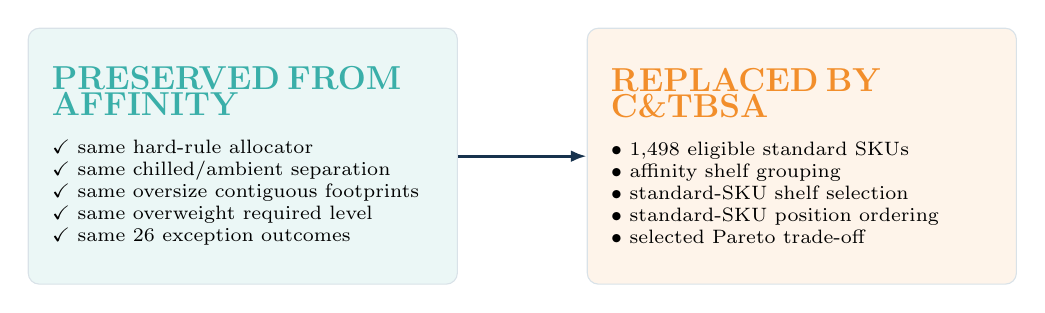
\begin{tikzpicture}[
    card/.style={rounded corners=4pt,draw=Mid,minimum width=5.45cm,
      minimum height=3.25cm,text width=4.85cm,align=left,font=\scriptsize},
    arr/.style={-{Latex[length=2mm]},very thick,Navy}
  ]
    \node[card,fill=Cyan!10] (keep) at (0,0) {
      {\large\color{Cyan}\bfseries PRESERVED FROM AFFINITY}\\[2mm]
      $\checkmark$ same hard-rule allocator\\
      $\checkmark$ same chilled/ambient separation\\
      $\checkmark$ same oversize contiguous footprints\\
      $\checkmark$ same overweight required level\\
      $\checkmark$ same 26 exception outcomes};
    \node[card,fill=Orange!10] (change) at (7.1,0) {
      {\large\color{Orange}\bfseries REPLACED BY C\&TBSA}\\[2mm]
      $\bullet$ 1,498 eligible standard SKUs\\
      $\bullet$ affinity shelf grouping\\
      $\bullet$ standard-SKU shelf selection\\
      $\bullet$ standard-SKU position ordering\\
      $\bullet$ selected Pareto trade-off};
    \draw[arr] (keep)--(change);
  \end{tikzpicture}
  \vspace{0.35cm}
  \begin{alertblock}{Meaning of ``same approach''}
    \centering\scriptsize Physical inventory is treated exactly as in Affinity.
    The complete final layout is intentionally different because C\&TBSA must
    re-cluster standard SKUs to optimize its two paper objectives.
  \end{alertblock}
\end{frame}

\begin{frame}{Step 1: turn order history into two simple scores}
  \begin{columns}[T,onlytextwidth]
    \column{0.47\textwidth}
    \begin{block}{Small example first}
      \scriptsize
      \begin{tabular}{@{}lcc@{}}
        \toprule
        \textbf{Store + day group} & \textbf{SKU 17} & \textbf{SKU 04}\\
        \midrule
        Store A, Monday & $\checkmark$ & $\checkmark$\\
        Store B, Monday & $\checkmark$ & --\\
        \bottomrule
      \end{tabular}
      \vspace{1mm}

      SKU 17 is requested in \textbf{2} groups.\\
      SKU 04 is requested in \textbf{1} group.\\
      They appear together in \textbf{1} group.
    \end{block}
    \begin{alertblock}{Plain-language question}
      \scriptsize How popular is each SKU, and how often are two SKUs requested
      together on the same store delivery day?
    \end{alertblock}
    \column{0.49\textwidth}
    \begin{block}{Mathematical proof used by the code}
      \[
        F_j=\sum_g X_{g,j},\qquad
        N_{jj'}=\sum_g X_{g,j}X_{g,j'}
      \]
      \scriptsize
      $g$ = one Store ID + Date group.\quad $j,j'$ = SKU indices.\\
      $X_{g,j}=1$ if group $g$ requests SKU $j$; otherwise $0$.\\
      Therefore: $F_{17}=2$, $F_{04}=1$, and $N_{17,04}=1$.
    \end{block}
    \centering
    \pill{Navy}{982,992 LINES} $\rightarrow$
    \pill{Blue}{12,398 GROUPS}\\[2mm]
    \pill{Cyan}{1,524 SKUs} $\rightarrow$
    \pill{Orange}{1,498 OPTIMIZED}
  \end{columns}
\end{frame}

\begin{frame}{Step 2: describe one possible shelf plan}
  \centering
  {\large\color{Navy}\bfseries Write every eligible SKU once, shuffle the list,
  then cut it into shelf-sized groups.}\par
  \vspace{0.32cm}
  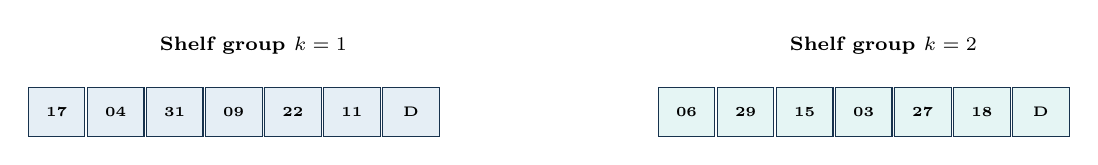
\begin{tikzpicture}[
    gene/.style={draw=Navy,minimum width=0.72cm,minimum height=0.62cm,
      font=\tiny\bfseries},
    shelf/.style={rounded corners=3pt,draw=Mid,fill=Light,inner sep=3mm}
  ]
    \node[shelf] (s1) at (0,0) {};
    \foreach \x/\lab in {-2.5/17,-1.75/04,-1/31,-0.25/09,0.5/22,1.25/11,2/D}
      \node[gene,fill=Blue!12] at (\x,0) {\lab};
    \node[above=3mm of s1,font=\scriptsize\bfseries] {Shelf group $k=1$};
    \node[shelf] (s2) at (8.0,0) {};
    \foreach \x/\lab in {5.5/06,6.25/29,7/15,7.75/03,8.5/27,9.25/18,10/D}
      \node[gene,fill=Cyan!13] at (\x,0) {\lab};
    \node[above=3mm of s2,font=\scriptsize\bfseries] {Shelf group $k=2$};
  \end{tikzpicture}
  \vspace{0.35cm}
  \begin{columns}[T,onlytextwidth]
    \column{0.31\textwidth}
      \begin{block}{No duplication}
        \centering\scriptsize Every SKU appears in exactly one group:
        $\sum_k x_{jk}=1$.
      \end{block}
    \column{0.31\textwidth}
      \begin{block}{No overfilling}
        \centering\scriptsize Shelf $k$ holds at most $Z_k$ locations:
        $\sum_j x_{jk}\le Z_k$.
      \end{block}
    \column{0.31\textwidth}
      \begin{block}{Unused space}
        \centering\scriptsize $D$ is a zero-demand dummy gene representing an
        empty shelf location.
      \end{block}
  \end{columns}
  {\tiny $x_{jk}=1$ means SKU $j$ is assigned to shelf group $k$; otherwise $0$.}
\end{frame}

\begin{frame}{Step 3: score every plan on two business goals}
  \begin{columns}[T,onlytextwidth]
    \column{0.48\textwidth}
    \begin{block}{Goal A: keep requested-together SKUs together}
      \centering
      \pill{Blue}{SKU 17} $+$ \pill{Cyan}{SKU 04}
      $\longrightarrow$ \pill{Green}{SAME SHELF}\\[2mm]
      \[
        \max f_1=\sum_{j<j'}\sum_k N_{jj'}x_{jk}x_{j'k}
      \]
      \scriptsize Larger $f_1$ means more frequently co-requested SKU pairs
      are stored on the same shelf.
    \end{block}
    \column{0.48\textwidth}
    \begin{block}{Goal B: avoid one shelf carrying most demand}
      \centering
      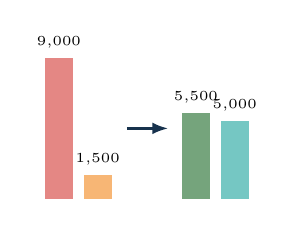
\begin{tikzpicture}[x=0.58cm,y=0.00020cm]
        \fill[Red!70] (0,0) rectangle (0.62,9000);
        \fill[Orange!65] (0.85,0) rectangle (1.47,1500);
        \draw[-{Latex[length=2mm]},thick,Navy] (1.8,4500)--(2.7,4500);
        \fill[Green!70] (3.0,0) rectangle (3.62,5500);
        \fill[Cyan!70] (3.85,0) rectangle (4.47,5000);
        \foreach \x/\v in {0.31/9000,1.16/1500,3.31/5500,4.16/5000}
          \node[above,font=\tiny] at (\x,\v) {\pgfmathprintnumber{\v}};
      \end{tikzpicture}
      \[
        W_k=\sum_j F_jx_{jk},\qquad \min f_2=W_{\max}
      \]
      \scriptsize $W_k$ is demand assigned to shelf $k$; $W_{\max}$ is the
      busiest shelf. Smaller $W_{\max}$ means a more even workload.
    \end{block}
  \end{columns}
  \begin{alertblock}{Important boundary}
    \centering\scriptsize These objectives balance \textbf{SKU grouping and
    shelf workload}. They do not directly minimize AMR trips, travel distance,
    queues, or shared-lane congestion.
  \end{alertblock}
\end{frame}

\begin{frame}{Step 4: let the computer improve many plans repeatedly}
  \centering
  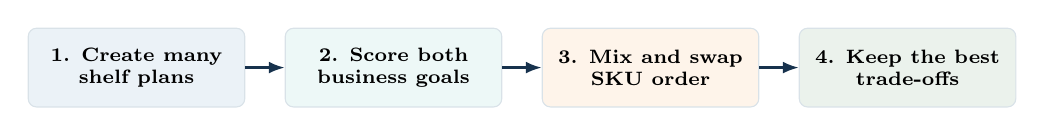
\begin{tikzpicture}[
    proc/.style={rounded corners=3pt,draw=Mid,fill=Light,minimum width=2.75cm,
      minimum height=1.0cm,align=center,font=\scriptsize\bfseries},
    arr/.style={-{Latex[length=2mm]},thick,Navy}
  ]
    \node[proc,fill=Blue!9] (make) {1. Create many\\shelf plans};
    \node[proc,fill=Cyan!9,right=5mm of make] (score) {2. Score both\\business goals};
    \node[proc,fill=Orange!10,right=5mm of score] (change) {3. Mix and swap\\SKU order};
    \node[proc,fill=Green!10,right=5mm of change] (keep) {4. Keep the best\\trade-offs};
    \foreach \a/\b in {make/score,score/change,change/keep}\draw[arr](\a)--(\b);
  \end{tikzpicture}
  \vspace{0.35cm}
  \begin{columns}[T,onlytextwidth]
    \column{0.52\textwidth}
    \begin{block}{Technical names, translated}
      \scriptsize
      \begin{tabular}{@{}p{0.24\textwidth}p{0.66\textwidth}@{}}
        \textbf{NSGA-II} & repeats the four-step search above\\
        \textbf{PMX} & combines two parent SKU orders without duplicating SKUs\\
        \textbf{2-opt swap} & exchanges two positions to create a new plan\\
        \textbf{Pareto set} & plans where neither goal can improve freely\\
      \end{tabular}
    \end{block}
    \column{0.44\textwidth}
    \begin{block}{Paper parameters}
      \centering\small
      $P=100,\ G=50{,}000$\\
      $P_c=0.9,\ P_m=0.1$
    \end{block}
    \begin{alertblock}{Current reproducible run}
      \centering\small
      $P=100,\ G=500$\\
      $P_c=0.9,\ P_m=0.1,\ \text{seed}=0$
    \end{alertblock}
  \end{columns}
  {\tiny $P$ = number of plans; $G$ = repeated generations; $P_c$ = PMX chance;
  $P_m$ = swap chance.}
\end{frame}

\begin{frame}{Step 5: choose a trade-off and place busy groups closer}
  \begin{columns}[T,onlytextwidth]
    \column{0.46\textwidth}
    \begin{block}{No single plan wins both goals}
      \centering
      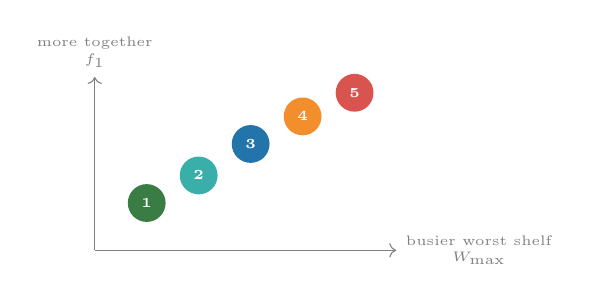
\begin{tikzpicture}[x=0.66cm,y=0.50cm]
        \draw[->,gray] (0,0)--(5.8,0)
          node[right,font=\tiny,align=center] {busier worst shelf\\$W_{\max}$};
        \draw[->,gray] (0,0)--(0,4.4)
          node[above,font=\tiny,align=center] {more together\\$f_1$};
        \foreach \x/\y/\n/\col in {1/1.2/1/Green,2/1.9/2/Cyan,3/2.7/3/Blue,
          4/3.4/4/Orange,5/4.0/5/Red}
          \node[circle,fill=\col,text=white,minimum size=0.48cm,
            inner sep=0pt,font=\tiny\bfseries] at (\x,\y) {\n};
      \end{tikzpicture}
      \scriptsize Five representative Pareto solutions are shown. The saved
      run selects \textbf{solution 5}, favouring co-request grouping.
    \end{block}
    \column{0.50\textwidth}
    \begin{block}{Then map groups to real shelves}
      \begin{enumerate}
        \item Calculate each group workload $W_k$.
        \item Rank groups from busiest to quietest.
        \item Rank eligible shelves from nearest to farthest.
        \item Match both rankings; randomize positions inside each shelf.
      \end{enumerate}
    \end{block}
    \centering
    \pill{Red}{BUSIEST GROUP}\\[1mm]
    $\downarrow$\\[1mm]
    \pill{Green}{NEAREST ELIGIBLE SHELF}
  \end{columns}
\end{frame}

\begin{frame}{Exactly what is reproduced, adapted, and not claimed}
  \scriptsize
  \begin{tabular}{@{}p{0.19\textwidth}p{0.34\textwidth}p{0.37\textwidth}@{}}
    \toprule
    & \textbf{Implemented meaning} & \textbf{Current status}\\
    \midrule
    \cellcolor{Green!12}\textbf{Paper method}
      & permutation chromosome; two objectives; NSGA-II; PMX; swap mutation;
        Pareto representatives; demand-ranked Stage 2
      & reproduced after the Affinity baseline; the paper search itself is unchanged\\[1mm]
    \cellcolor{Blue!10}\textbf{Warehouse adaptation}
      & AMR shelf as storage area; 12 locations; ambient/chilled strata;
        fixed physical exceptions; dummy empty genes
      & feasibility added without inserting lane load into the paper objectives\\[1mm]
    \cellcolor{Orange!12}\textbf{Static validation}
      & Store ID + Date shelf visits routed over the saved grid to service endpoints
      & heatmaps, peak, P95, expected travel, and relocation report\\[1mm]
    \cellcolor{Red!10}\textbf{Not reproduced yet}
      & fleet dispatch, queues, blocking, collisions, picking delay, throughput
      & no simulation validation; no operational throughput claim\\
    \bottomrule
  \end{tabular}
  \vspace{0.35cm}
  \begin{alertblock}{Interpretation boundary}
    A lower $W_{\max}$ proves a more balanced assignment-demand objective.
    It does not prove that total lane traffic or travel decreased.
  \end{alertblock}
  \source{Lee, Chung, and Yoon, C\&TBSA, DOI: 10.1016/j.cie.2019.106129.}
\end{frame}

\begin{frame}{Implementation proof: the traffic-balance objective is active}
  \begin{columns}[T,onlytextwidth]
    \column{0.37\textwidth}
    \begin{block}{What the optimizer calculates}
      \[
        W_k=\sum_jF_jx_{jk}
      \]
      \[
        \boxed{\min W_{\max}},\qquad
        W_{\max}=\max_kW_k
      \]
      \scriptsize $W_k$ is expected pickup demand assigned to shelf cluster
      $k$. Lower $W_{\max}$ means less demand concentrated in the busiest
      cluster.
    \end{block}
    \begin{alertblock}{How to read the evidence}
      \scriptsize Moving from solution 1 to solution 5 increases correlation,
      but also increases the maximum cluster demand. This is the intended
      Pareto trade-off from the paper.
    \end{alertblock}
    \column{0.59\textwidth}
    \begin{block}{Saved run: five actual Pareto representatives}
      \centering\scriptsize
      \begin{tabular}{@{}crrrr@{}}
        \toprule
        & \multicolumn{2}{c}{\textbf{Ambient}} &
          \multicolumn{2}{c}{\textbf{Chilled}}\\
        \textbf{Sol.} & $W_{\max}$ & \textbf{Correlation} &
          $W_{\max}$ & \textbf{Correlation}\\
        \midrule
        \cellcolor{Green!14}1 & \cellcolor{Green!14}\textbf{9,745} & 419,521 &
          \cellcolor{Green!14}\textbf{5,852} & 31,335\\
        2 & 10,467 & 432,044 & 7,378 & 39,540\\
        3 & 11,351 & 479,335 & 8,701 & 49,397\\
        4 & 12,031 & 499,629 & 10,547 & 58,838\\
        \cellcolor{Orange!14}5 & 14,096 & \cellcolor{Orange!14}\textbf{520,396} &
          14,188 & \cellcolor{Orange!14}\textbf{66,008}\\
        \bottomrule
      \end{tabular}
    \end{block}
    \centering
    \pill{Green}{SOLUTION 1: MORE TRAFFIC BALANCE}
    $\longrightarrow$
    \pill{Orange}{SOLUTION 5: MORE CORRELATION}\\[2mm]
    {\scriptsize Current saved layout uses \textbf{solution 5}; solution 3 is
    the clearer middle trade-off for the full demonstration.}
  \end{columns}
  \source{Values read from the ambient and chilled Pareto rows in the saved Traffic-Aware layout.}
\end{frame}

\begin{frame}{Paper component not implemented: operational simulation}
  \centering
  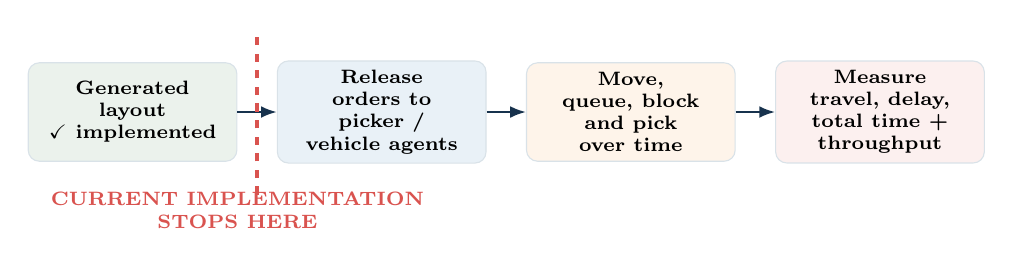
\begin{tikzpicture}[
    stage/.style={rounded corners=4pt,draw=Mid,minimum width=2.65cm,
      minimum height=1.25cm,text width=2.25cm,align=center,font=\scriptsize\bfseries},
    arr/.style={-{Latex[length=2mm]},thick,Navy}
  ]
    \node[stage,fill=Green!10] (layout) {Generated layout\\\checkmark\ implemented};
    \node[stage,fill=Blue!10,right=5mm of layout] (orders) {Release orders to\\picker / vehicle agents};
    \node[stage,fill=Orange!10,right=5mm of orders] (move) {Move, queue, block\\and pick over time};
    \node[stage,fill=Red!9,right=5mm of move] (measure) {Measure travel, delay,\\total time + throughput};
    \foreach \a/\b in {layout/orders,orders/move,move/measure}\draw[arr](\a)--(\b);
    \draw[Red,very thick,dashed] ($(layout.east)!0.5!(orders.west)+(0,-1.05)$)
      -- ($(layout.east)!0.5!(orders.west)+(0,1.05)$);
    \node[below=9mm of layout.east,anchor=north,font=\scriptsize\bfseries,
      text=Red,align=center] {CURRENT IMPLEMENTATION\\STOPS HERE};
  \end{tikzpicture}
  \vspace{0.45cm}
  \begin{columns}[T,onlytextwidth]
    \column{0.48\textwidth}
    \begin{block}{Missing operational behaviour}
      \scriptsize
      \begin{itemize}
        \item picker / AMR dispatch and order release timing;
        \item aisle occupancy, queues, blocking and conflicts;
        \item movement speed, picking/service time and station waiting;
        \item repeated stochastic runs with different random seeds.
      \end{itemize}
    \end{block}
    \column{0.48\textwidth}
    \begin{alertblock}{What cannot yet be claimed}
      \scriptsize We can prove a lower cluster-demand proxy $W_{\max}$. We
      cannot yet prove lower congestion delay, faster order completion, or
      higher throughput. The current heatmap is static expected flow, not a
      time-dependent simulation.
    \end{alertblock}
  \end{columns}
\end{frame}

\begin{frame}{Development needed for a complete Traffic-Aware demonstration}
  \centering
  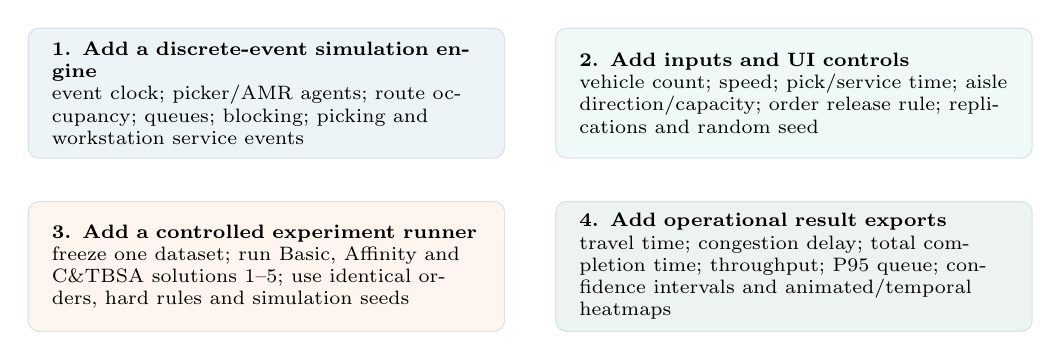
\begin{tikzpicture}[
    work/.style={rounded corners=4pt,draw=Mid,minimum width=6.05cm,
      minimum height=1.65cm,text width=5.45cm,align=left,font=\scriptsize},
    tag/.style={font=\scriptsize\bfseries,text=white,rounded corners=2pt,
      inner sep=2mm}
  ]
    \node[work,fill=Blue!8] (engine) at (0,1.15)
      {\textbf{1. Add a discrete-event simulation engine}\\
       event clock; picker/AMR agents; route occupancy; queues; blocking;
       picking and workstation service events};
    \node[work,fill=Cyan!8] (inputs) at (6.7,1.15)
      {\textbf{2. Add inputs and UI controls}\\
       vehicle count; speed; pick/service time; aisle direction/capacity;
       order release rule; replications and random seed};
    \node[work,fill=Orange!8] (runner) at (0,-1.05)
      {\textbf{3. Add a controlled experiment runner}\\
       freeze one dataset; run Basic, Affinity and C\&TBSA solutions 1--5;
       use identical orders, hard rules and simulation seeds};
    \node[work,fill=Green!9] (report) at (6.7,-1.05)
      {\textbf{4. Add operational result exports}\\
       travel time; congestion delay; total completion time; throughput;
       P95 queue; confidence intervals and animated/temporal heatmaps};
  \end{tikzpicture}
  \vspace{0.3cm}
  \begin{block}{Code areas to extend}
    \centering\scriptsize
    \texttt{traffic.py}: simulation adapter and experiment metrics \quad
    \texttt{gui.py}: controls, run/cancel and result views\\
    new \texttt{traffic\_simulation.py}: event engine \quad
    new \texttt{traffic\_experiment.py}: repeatable multi-layout comparison
  \end{block}
  \begin{alertblock}{Keep the paper method intact}
    \centering\scriptsize Do not insert lane congestion into the C\&TBSA
    objective when claiming paper replication. Use simulation to validate each
    Pareto layout, as the paper does.
  \end{alertblock}
\end{frame}

\begin{frame}{Full demonstration: compare three layout-generation methods fairly}
  \centering
  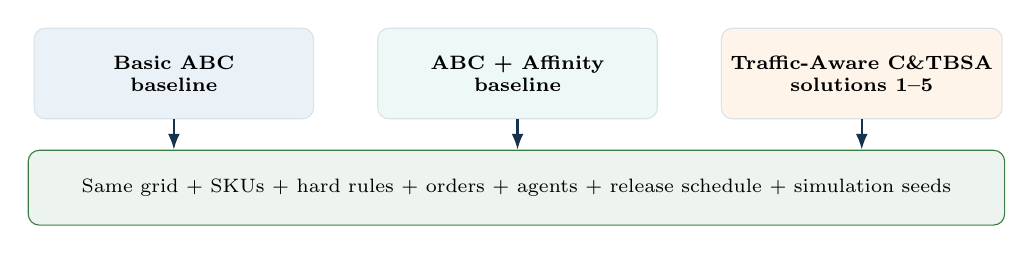
\begin{tikzpicture}[
    method/.style={rounded corners=4pt,draw=Mid,minimum width=3.55cm,
      minimum height=1.15cm,align=center,font=\scriptsize\bfseries},
    arr/.style={-{Latex[length=2mm]},thick,Navy}
  ]
    \node[method,fill=Blue!9] (basic) {Basic ABC\\baseline};
    \node[method,fill=Cyan!9,right=8mm of basic] (aff) {ABC + Affinity\\baseline};
    \node[method,fill=Orange!10,right=8mm of aff] (traffic)
      {Traffic-Aware C\&TBSA\\solutions 1--5};
    \node[rounded corners=4pt,draw=Green,fill=Green!9,minimum width=12.4cm,
      minimum height=0.95cm,align=center,font=\scriptsize] (frozen) at (4.35,-1.45)
      {Same grid + SKUs + hard rules + orders + agents + release schedule + simulation seeds};
    \foreach \m in {basic,aff,traffic}\draw[arr](\m.south)--(frozen.north -| \m.south);
  \end{tikzpicture}
  \vspace{0.35cm}
  \begin{columns}[T,onlytextwidth]
    \column{0.47\textwidth}
    \begin{block}{Optimization-level evidence}
      \scriptsize
      \begin{itemize}
        \item maximum cluster demand $W_{\max}$;
        \item co-request correlation $f_1$;
        \item shelves per order and occupied shelves;
        \item static travel and route-load heatmaps.
      \end{itemize}
    \end{block}
    \column{0.49\textwidth}
    \begin{block}{Operational simulation evidence}
      \scriptsize
      \begin{itemize}
        \item mean and P95 travel time;
        \item mean and P95 congestion delay;
        \item total order time $T= T_{travel}+T_{pick}+T_{delay}$;
        \item throughput and 95\% confidence interval.
      \end{itemize}
    \end{block}
  \end{columns}
  \begin{alertblock}{Decision rule}
    \centering\scriptsize Select the layout that improves total operational
    time without unacceptable travel, congestion, relocation, or hard-rule
    violations---not simply the layout with the lowest $W_{\max}$.
  \end{alertblock}
\end{frame}

\begin{frame}{Notation reference: C\&TBSA and global model}
  \scriptsize
  \begin{tabular}{@{}p{0.18\textwidth}p{0.74\textwidth}@{}}
    \toprule
    \textbf{Symbol} & \textbf{Meaning}\\
    \midrule
    $g$ & Fulfilment group: one unique (Store ID, Date) pair.\\
    $j,j'$ & Two different SKU indices; $j<j'$ counts each SKU pair once.\\
    $k$ & C\&TBSA cluster index; mapped here to one eligible AMR shelf.\\
    $X_{g,j}$ & Binary presence: 1 when group $g$ requests SKU $j$; otherwise 0.\\
    $F_j$ & Demand for SKU $j$: number of selected groups containing it.\\
    $N_{jj'}$ & Number of selected groups containing both SKUs $j$ and $j'$.\\
    $x_{jk}$ & Binary assignment: 1 if SKU $j$ belongs to cluster $k$; otherwise 0.\\
    $Z_k$ & Storage locations available in cluster/shelf $k$; here at most 12.\\
    $W_k,W_{\max}$ & Assigned cluster demand; maximum demand across all clusters.\\
    $f_1,f_2$ & Correlation-maximization and maximum-demand-minimization objectives.\\
    $P,G,P_c,P_m$ & Population, generations, PMX probability, and swap-mutation probability.\\
    $u_i,\ell_r$ & Complete handling unit $i$ and candidate location $r$ in global CP-SAT.\\
    \bottomrule
  \end{tabular}
\end{frame}

% 14
\begin{frame}{Global approach: assign all units together}
  \textcolor{Red}{\textbf{Decision:}} Which compatible location should
  \textbf{every complete unit} occupy in the final layout?
  \vspace{0.15cm}
  \begin{columns}[T,onlytextwidth]
    \column{0.55\textwidth}
  \centering
  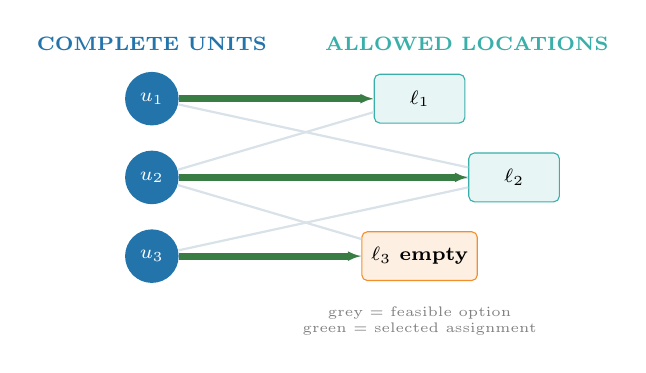
\begin{tikzpicture}[
    unit/.style={circle,fill=Blue,text=white,minimum size=0.68cm,font=\scriptsize\bfseries},
    loc/.style={rounded corners=2pt,draw=Cyan,fill=Cyan!12,minimum width=1.15cm,
      minimum height=0.62cm,font=\scriptsize\bfseries},
    possible/.style={Mid,line width=0.8pt},
    chosen/.style={Green,line width=2.5pt,-{Latex[length=1.7mm]}}
  ]
    \node[font=\scriptsize\bfseries,text=Blue] at (0,2.0) {COMPLETE UNITS};
    \node[unit] (u1) at (0,1.3) {$u_1$};
    \node[unit] (u2) at (0,0.3) {$u_2$};
    \node[unit] (u3) at (0,-0.7) {$u_3$};
    \node[font=\scriptsize\bfseries,text=Cyan] at (4.0,2.0) {ALLOWED LOCATIONS};
    \node[loc] (l1) at (3.4,1.3) {$\ell_1$};
    \node[loc] (l2) at (4.6,0.3) {$\ell_2$};
    \node[loc,fill=Orange!13,draw=Orange] (l3) at (3.4,-0.7) {$\ell_3$ empty};
    \foreach \a/\b in {u1/l1,u1/l2,u2/l1,u2/l2,u2/l3,u3/l2,u3/l3}
      \draw[possible] (\a)--(\b);
    \draw[chosen] (u1)--(l1);
    \draw[chosen] (u2)--(l2);
    \draw[chosen] (u3)--(l3);
    \node[below=2mm of l3,font=\tiny,text=gray,align=center]
      {grey = feasible option\\green = selected assignment};
  \end{tikzpicture}
    \column{0.41\textwidth}
    \begin{block}{CP-SAT model}
      \scriptsize
      \begin{enumerate}
        \item Remove locations that fail hard rules.
        \item Assign each unit once and use each location at most once.
        \item Calculate traffic for the whole assignment.
        \item Keep the best solution found within the time limit.
      \end{enumerate}
    \end{block}
    \vspace{0.15cm}
    {\scriptsize\color{Green!70!black}\bfseries Enables:}
    {\scriptsize empty-buffer moves, pair swaps, and multi-unit cycles in one model.}
  \end{columns}
  \vfill
  \centering
  \pill{Blue}{ONE UNIT PER LOCATION}\qquad
  \pill{Green}{WHOLE LAYOUT EVALUATED}
\end{frame}

% 15
\begin{frame}{How the global optimizer chooses the winner}
  \centering
  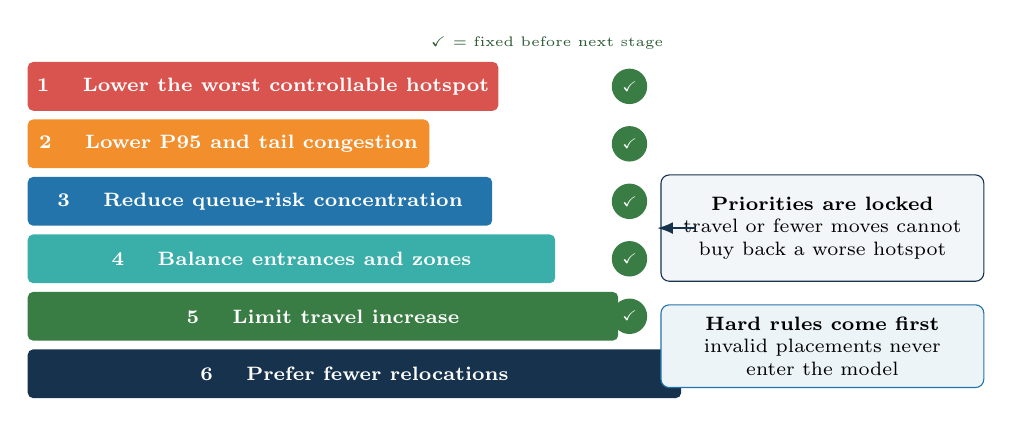
\begin{tikzpicture}[
    stage/.style={rounded corners=2pt,minimum height=0.62cm,align=left,
      text=white,font=\scriptsize\bfseries,anchor=west},
    checkpoint/.style={circle,fill=Green,text=white,minimum size=0.45cm,
      inner sep=0pt,font=\tiny\bfseries}
  ]
    \node[stage,fill=Red,minimum width=4.3cm] (s1) at (0,3.45) {1 \quad Lower the worst controllable hotspot};
    \node[stage,fill=Orange,minimum width=5.1cm] (s2) at (0,2.72) {2 \quad Lower P95 and tail congestion};
    \node[stage,fill=Blue,minimum width=5.9cm] (s3) at (0,1.99) {3 \quad Reduce queue-risk concentration};
    \node[stage,fill=Cyan,minimum width=6.7cm] (s4) at (0,1.26) {4 \quad Balance entrances and zones};
    \node[stage,fill=Green,minimum width=7.5cm] (s5) at (0,0.53) {5 \quad Limit travel increase};
    \node[stage,fill=Navy,minimum width=8.3cm] (s6) at (0,-0.20) {6 \quad Prefer fewer relocations};
    \foreach \y in {3.45,2.72,1.99,1.26,0.53}
      \node[checkpoint] at (7.65,\y) {$\checkmark$};
    \node[font=\tiny,text=Green!70!black,anchor=east] at (8.2,4.0)
      {$\checkmark$ = fixed before next stage};
    \node[rounded corners=3pt,draw=Navy,fill=Light,minimum width=4.1cm,
      minimum height=1.35cm,align=center,font=\scriptsize] at (10.1,1.65)
      {\textbf{Priorities are locked}\\
       travel or fewer moves cannot\\
       buy back a worse hotspot};
    \draw[-{Latex[length=2mm]},thick,Navy] (8.5,1.65)--(8.0,1.65);
    \node[rounded corners=3pt,draw=Blue,fill=Blue!8,minimum width=4.1cm,
      minimum height=1.05cm,align=center,font=\scriptsize] at (10.1,0.15)
      {\textbf{Hard rules come first}\\
       invalid placements never\\
       enter the model};
  \end{tikzpicture}
  \vfill
  {\scriptsize The solver records \textbf{OPTIMAL} only with proof. A
  time-limited valid result is \textbf{FEASIBLE}, with its bound or gap reported.}
\end{frame}

% 16
\begin{frame}{Traffic-aware or global: which one should we use?}
  \begin{center}
  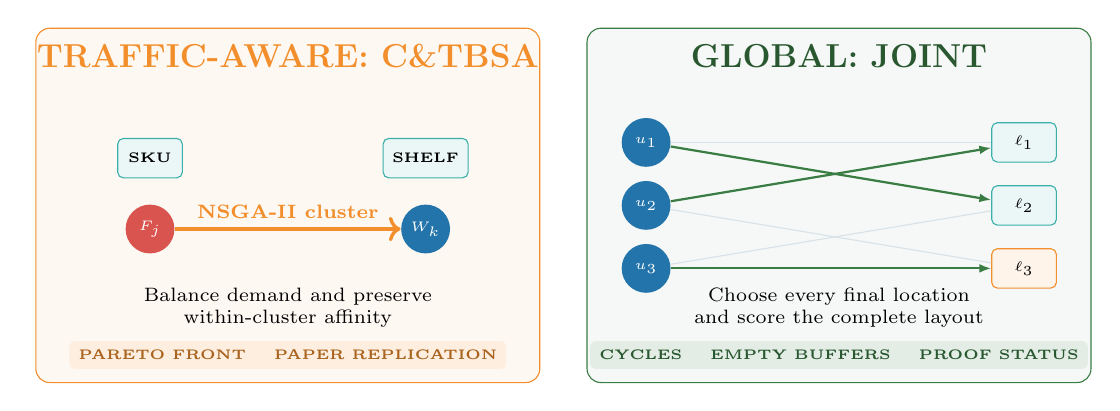
\begin{tikzpicture}[
    unit/.style={circle,fill=Blue,text=white,minimum size=0.62cm,
      inner sep=0pt,font=\tiny\bfseries},
    loc/.style={rounded corners=2pt,draw=Cyan,fill=Cyan!10,
      minimum width=0.82cm,minimum height=0.5cm,font=\tiny\bfseries},
    arr/.style={-{Latex[length=1.5mm]},thick}
  ]
    \draw[rounded corners=5pt,draw=Orange,fill=Orange!6]
      (-0.2,-2.1) rectangle (6.2,2.4);
    \node[font=\large\bfseries,text=Orange] at (3.0,2.05)
      {TRAFFIC-AWARE: C\&TBSA};
    \node[loc] (la) at (1.25,0.75) {SKU};
    \node[loc] (lb) at (4.75,0.75) {SHELF};
    \node[unit,fill=Red] (lu) at (1.25,-0.15) {$F_j$};
    \node[unit] (lv) at (4.75,-0.15) {$W_k$};
    \draw[->,very thick,Orange] (lu)--node[above,font=\scriptsize\bfseries]
      {NSGA-II cluster}(lv);
    \node[align=center,font=\scriptsize] at (3.0,-1.15)
      {Balance demand and preserve\\within-cluster affinity};
    \node[rounded corners=2pt,fill=Orange!15,text=Orange!70!black,
      font=\tiny\bfseries] at (3.0,-1.75) {PARETO FRONT \quad PAPER REPLICATION};

    \draw[rounded corners=5pt,draw=Green,fill=Green!5]
      (6.8,-2.1) rectangle (13.2,2.4);
    \node[font=\large\bfseries,text=Green!70!black] at (10.0,2.05)
      {GLOBAL: JOINT};
    \node[unit] (gu1) at (7.55,0.95) {$u_1$};
    \node[unit] (gu2) at (7.55,0.15) {$u_2$};
    \node[unit] (gu3) at (7.55,-0.65) {$u_3$};
    \node[loc] (gl1) at (12.35,0.95) {$\ell_1$};
    \node[loc] (gl2) at (12.35,0.15) {$\ell_2$};
    \node[loc,draw=Orange,fill=Orange!10] (gl3) at (12.35,-0.65) {$\ell_3$};
    \foreach \a/\b in {gu1/gl1,gu1/gl2,gu2/gl1,gu2/gl3,gu3/gl2,gu3/gl3}
      \draw[Mid] (\a)--(\b);
    \draw[arr,Green] (gu1)--(gl2);
    \draw[arr,Green] (gu2)--(gl1);
    \draw[arr,Green] (gu3)--(gl3);
    \node[align=center,font=\scriptsize] at (10.0,-1.15)
      {Choose every final location\\and score the complete layout};
    \node[rounded corners=2pt,fill=Green!14,text=Green!70!black,
      font=\tiny\bfseries] at (10.0,-1.75) {CYCLES \quad EMPTY BUFFERS \quad PROOF STATUS};
  \end{tikzpicture}
  \end{center}
  \vspace{0.15cm}
  \begin{block}{Choose according to the research question}
    \centering
    \begin{minipage}{0.47\linewidth}
      \centering\textbf{C\&TBSA}\\
      \scriptsize Reproduce correlation + workload balance
    \end{minipage}\hfill
    \begin{minipage}{0.47\linewidth}
      \centering\textbf{Global CP-SAT}\\
      \scriptsize Optimize mapped lane loads
    \end{minipage}
  \end{block}
  \centering
  {\tiny C\&TBSA follows the paper's two-stage method. Global CP-SAT is our
  separate warehouse-specific model; its objective directly uses the grid network.}
\end{frame}

% 17
\begin{frame}{Current evidence: saved global run}
  \centering
  \metric{Green}{-2.38\%}{controllable-resource peak}
  \hfill
  \metric{Blue}{0.00\%}{nearest-rank controllable P95 change}
  \hfill
  \metric{Cyan}{-0.01\%}{expected travel}
  \vspace{0.4cm}
  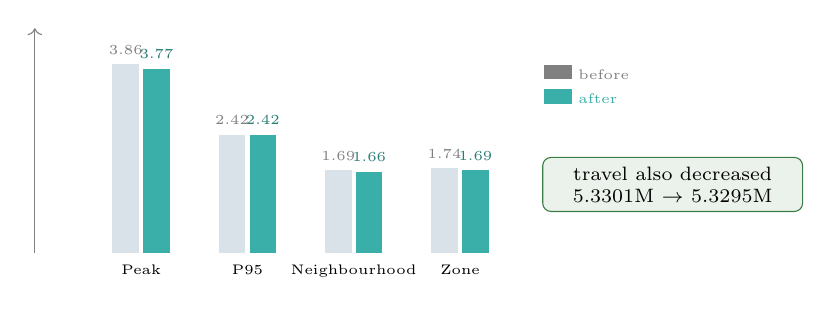
\begin{tikzpicture}[x=1.35cm,y=0.62cm]
    \draw[->,gray] (0,0)--(0,4.6);
    \foreach \x/\lab/\before/\after in {
      1/Peak/3.86/3.77,
      2/P95/2.42/2.42,
      3/Neighbourhood/1.69/1.66,
      4/Zone/1.74/1.69}{
      \fill[Mid] (\x-0.27,0) rectangle (\x-0.02,\before);
      \fill[Cyan] (\x+0.02,0) rectangle (\x+0.27,\after);
      \node[below,font=\tiny,align=center] at (\x,-0.05) {\lab};
      \node[above,font=\tiny,text=gray] at (\x-0.145,\before) {\before};
      \node[above,font=\tiny,text=Cyan!70!black] at (\x+0.145,\after) {\after};
    }
    \node[anchor=west,font=\tiny,text=gray] at (4.7,3.7) {\rule{0.35cm}{0.18cm} before};
    \node[anchor=west,font=\tiny,text=Cyan!70!black] at (4.7,3.2)
      {\color{Cyan}\rule{0.35cm}{0.18cm} after};
    \node[rounded corners=3pt,draw=Green,fill=Green!10,align=center,
      font=\scriptsize,minimum width=3.3cm] at (6.0,1.4)
      {travel also decreased\\5.3301M $\rightarrow$ 5.3295M};
  \end{tikzpicture}
  \vspace{0.2cm}

  {\scriptsize 128 handling units, 158 candidate locations, 7,917 binary
  variables, 31 relocated units; 180 s result status: \textbf{FEASIBLE}.}
  \source{\texttt{resources/map/global\_traffic\_optimized\_layout.slotting.json}. Relative loads are not physical utilization because the network has no explicit capacities.}
\end{frame}

% 18
\begin{frame}{Validation logic and interpretation boundary}
  \centering
  
\begin{tikzpicture}[
    check/.style={rounded corners=3pt,draw=Green,fill=Green!10,
      minimum width=1.85cm,minimum height=1.0cm,align=center,font=\scriptsize\bfseries},
    arr/.style={-{Latex[length=2mm]},thick,Navy}
  ]
    \node[check] (c1) {Membership\\unchanged};
    \node[check,right=2mm of c1] (c2) {Unique\\addresses};
    \node[check,right=2mm of c2] (c3) {Hard rules\\pass};
    \node[check,right=2mm of c3] (c4) {P95 + spatial\\guards pass};
    \node[check,right=2mm of c4] (c5) {Status + gap\\recorded};
    \foreach \a/\b in {c1/c2,c2/c3,c3/c4,c4/c5}\draw[arr](\a)--(\b);
    \node[rounded corners=4pt,fill=Green,text=white,minimum width=1.85cm,
      minimum height=0.9cm,font=\scriptsize\bfseries,right=3mm of c5] (accept)
      {ACCEPT LAYOUT};
    \draw[arr](c5)--(accept);
  \end{tikzpicture}
  \vspace{0.8cm}
  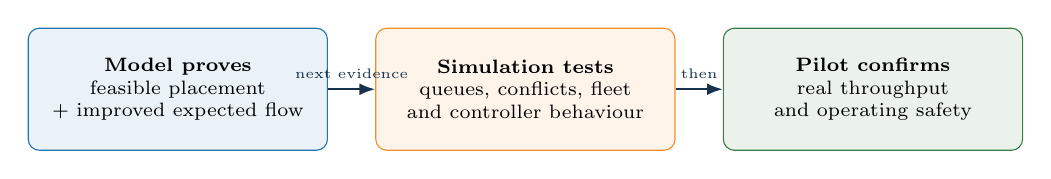
\begin{tikzpicture}[
    model/.style={rounded corners=4pt,draw=Blue,fill=Blue!9,
      minimum width=3.8cm,minimum height=1.55cm,align=center,font=\scriptsize},
    real/.style={rounded corners=4pt,draw=Orange,fill=Orange!10,
      minimum width=3.8cm,minimum height=1.55cm,align=center,font=\scriptsize},
    arr/.style={-{Latex[length=2mm]},thick,Navy}
  ]
    \node[model] (m) {\textbf{Model proves}\\feasible placement\\+ improved expected flow};
    \node[real,right=0.6cm of m] (s) {\textbf{Simulation tests}\\queues, conflicts, fleet\\and controller behaviour};
    \node[real,right=0.6cm of s,draw=Green,fill=Green!10] (p)
      {\textbf{Pilot confirms}\\real throughput\\and operating safety};
    \draw[arr](m)--node[above,font=\tiny]{next evidence}(s);
    \draw[arr](s)--node[above,font=\tiny]{then}(p);
  \end{tikzpicture}
\end{frame}

% 19
\begin{frame}{Next progress milestone}
  \centering
  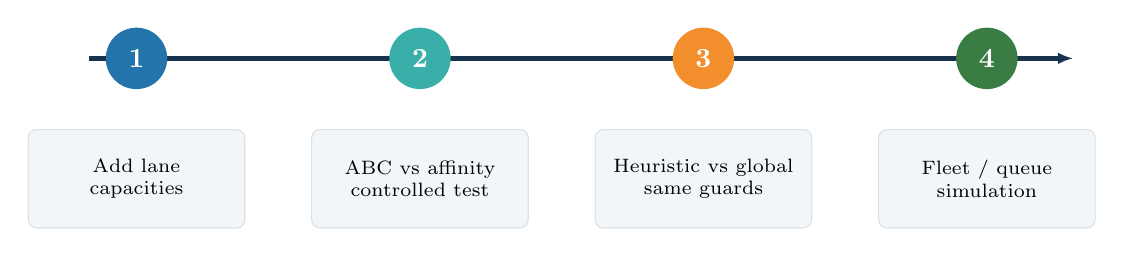
\begin{tikzpicture}[
    mile/.style={circle,minimum size=0.78cm,text=white,font=\bfseries},
    card/.style={rounded corners=3pt,draw=Mid,fill=Light,minimum width=2.75cm,
      minimum height=1.25cm,align=center,font=\scriptsize},
    arr/.style={-{Latex[length=2mm]},line width=2pt,Navy}
  ]
    \draw[arr] (0,1.8)--(12.5,1.8);
    \foreach \x/\num/\col/\txt in {
      0.6/1/Blue/{Add lane\\capacities},
      4.2/2/Cyan/{ABC vs affinity\\controlled test},
      7.8/3/Orange/{Heuristic vs global\\same guards},
      11.4/4/Green/{Fleet / queue\\simulation}}{
      \node[mile,fill=\col] (m\num) at (\x,1.8) {\num};
      \node[card,below=5mm of m\num] {\txt};
    }
  \end{tikzpicture}
  \vspace{0.7cm}
  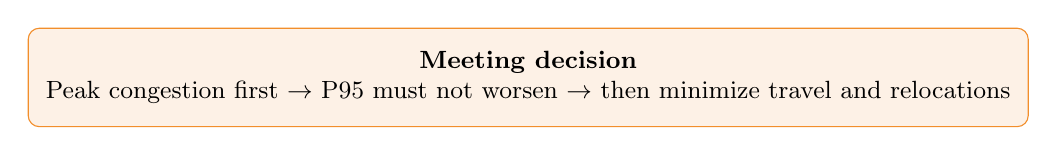
\begin{tikzpicture}
    \node[rounded corners=4pt,fill=Orange!12,draw=Orange,minimum width=12.7cm,
      minimum height=1.25cm,align=center,font=\small]
      {\textbf{Meeting decision}\\
       Peak congestion first $\rightarrow$ P95 must not worsen
       $\rightarrow$ then minimize travel and relocations};
  \end{tikzpicture}
  \vfill
  {\large\color{Navy}\bfseries Implemented approach $\rightarrow$ controlled comparative validation}
\end{frame}

\section{Three-layout result comparison}

\begin{frame}{Comparison protocol: three saved layouts, one measurement method}
  \centering
  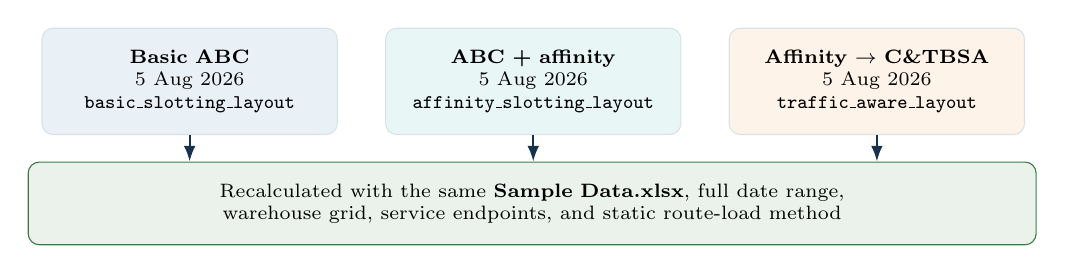
\begin{tikzpicture}[
    card/.style={rounded corners=4pt,minimum width=3.75cm,minimum height=1.35cm,
      text width=3.35cm,align=center,font=\scriptsize,draw=Mid},
    arr/.style={-{Latex[length=2mm]},thick,Navy}
  ]
    \node[card,fill=Blue!10] (basic) {\textbf{Basic ABC}\\5 Aug 2026\\\texttt{basic\_slotting\_layout}};
    \node[card,fill=Cyan!11,right=6mm of basic] (aff) {\textbf{ABC + affinity}\\5 Aug 2026\\\texttt{affinity\_slotting\_layout}};
    \node[card,fill=Orange!11,right=6mm of aff] (ctbsa) {\textbf{Affinity $\rightarrow$ C\&TBSA}\\5 Aug 2026\\\texttt{traffic\_aware\_layout}};
    \node[rounded corners=4pt,draw=Green,fill=Green!10,
      minimum width=12.8cm,minimum height=1.05cm,text width=12.1cm,
      align=center,font=\scriptsize]
      (common) at (4.35,-1.55)
      {Recalculated with the same \textbf{Sample Data.xlsx}, full date range,
       warehouse grid, service endpoints, and static route-load method};
    \foreach \a in {basic,aff,ctbsa}\draw[arr](\a.south)--(common.north -| \a.south);
  \end{tikzpicture}
  \vspace{0.35cm}
  \begin{alertblock}{Controlled static comparison}
    \scriptsize All three layouts now use the same canonical grid, SKU/chilled
    inputs, order workbook, hard-rule profile, and route calculation. Each
    assigns 1,523 SKUs and excludes the same dimension-incompatible SKU 139112.
    This is static expected-flow evidence, not simulation or throughput proof.
  \end{alertblock}
\end{frame}

\begin{frame}{Assignment coverage and warehouse-space use}
  \small
  \centering
  \begin{tabular}{@{}lrrr@{}}
    \toprule
    \textbf{Metric} & \textbf{Basic ABC} & \textbf{Affinity} & \textbf{C\&TBSA S5}\\
    \midrule
    Input SKUs & 1,524 & 1,524 & 1,524\\
    Assigned SKUs & 1,523 & 1,523 & 1,523\\
    Unassigned SKUs & 1 & 1 & 1\\
    Occupied shelves & \cellcolor{Green!12}132 & \cellcolor{Green!12}132 & 158\\
    Mean SKUs / occupied shelf & \cellcolor{Green!12}11.54 & \cellcolor{Green!12}11.54 & 9.64\\
    ABC-pure shelf fraction & \cellcolor{Green!12}95.5\% & 74.2\% & 5.7\%\\
    Mixed-ABC shelves & \cellcolor{Green!12}6 & 34 & 149\\
    \bottomrule
  \end{tabular}
  \vspace{0.45cm}
  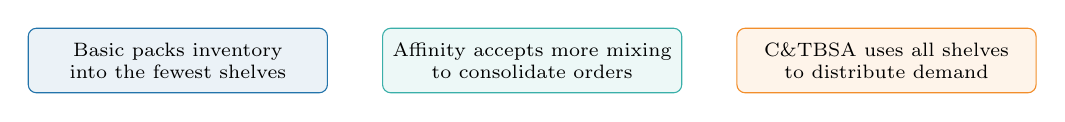
\begin{tikzpicture}[
    note/.style={rounded corners=3pt,minimum width=3.8cm,minimum height=0.82cm,
      align=center,font=\scriptsize}
  ]
    \node[note,draw=Blue,fill=Blue!9] at (0,0)
      {Basic packs inventory\\into the fewest shelves};
    \node[note,draw=Cyan,fill=Cyan!9] at (4.5,0)
      {Affinity accepts more mixing\\to consolidate orders};
    \node[note,draw=Orange,fill=Orange!10] at (9.0,0)
      {C\&TBSA uses all shelves\\to distribute demand};
  \end{tikzpicture}
\end{frame}

\begin{frame}{C\&TBSA succeeds at its shelf-demand balancing objective}
  \begin{columns}[T,onlytextwidth]
    \column{0.52\textwidth}
    \centering
    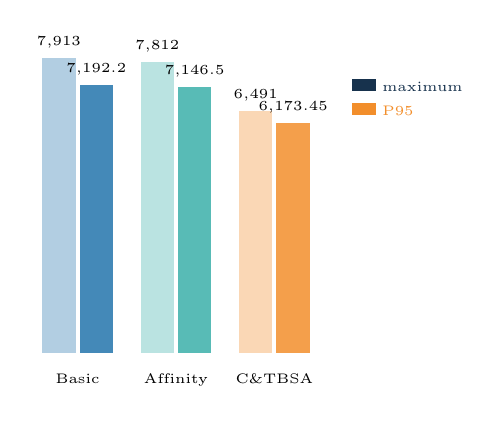
\begin{tikzpicture}[x=1.25cm,y=0.00048cm]
      \foreach \x/\lab/\max/\p/\col in {
        0/Basic/7913/7192.2/Blue,
        1/Affinity/7812/7146.5/Cyan,
        2/C\&TBSA/6491/6173.45/Orange}{
        \fill[\col!35] (\x,0) rectangle (\x+0.34,\max);
        \fill[\col!85] (\x+0.38,0) rectangle (\x+0.72,\p);
        \node[below,font=\tiny,align=center] at (\x+0.36,-300) {\lab};
        \node[above,font=\tiny] at (\x+0.17,\max) {\pgfmathprintnumber{\max}};
        \node[above,font=\tiny] at (\x+0.55,\p) {\pgfmathprintnumber{\p}};
      }
      \node[anchor=west,font=\tiny] at (3.05,7200) {\color{Navy}\rule{0.3cm}{0.16cm} maximum};
      \node[anchor=west,font=\tiny] at (3.05,6550) {\color{Orange}\rule{0.3cm}{0.16cm} P95};
    \end{tikzpicture}
    \column{0.44\textwidth}
    \begin{block}{Measured shelf visits}
      \begin{tabular}{@{}lrr@{}}
        \toprule
        & \textbf{Maximum} & \textbf{CV}\\
        \midrule
        Basic & 7,913 & 0.700\\
        Affinity & 7,812 & 0.708\\
        C\&TBSA & \cellcolor{Green!15}\textbf{6,491} & \cellcolor{Green!15}\textbf{0.537}\\
        \bottomrule
      \end{tabular}
    \end{block}
    \begin{alertblock}{Result versus basic}
      \centering
      \textbf{18.0\% lower maximum}\par
      \textbf{23.3\% lower CV}
    \end{alertblock}
  \end{columns}
  \vspace{0.15cm}
  {\scriptsize $CV=\sigma_v/\bar v$; $v$ is expected visits to one shelf,
  $\bar v$ its mean, and $\sigma_v$ its standard deviation. Lower is more even.}
\end{frame}

\begin{frame}{But shelf balance increased total retrieval and route load}
  \scriptsize
  \centering
  \begin{tabular}{@{}lrrr@{}}
    \toprule
    \textbf{Metric (lower is better)} & \textbf{Basic ABC} & \textbf{Affinity} & \textbf{C\&TBSA S5}\\
    \midrule
    Total shelf visits & 441,862 & \cellcolor{Green!15}\textbf{432,668} & \cellcolor{Red!10}547,519\\
    Average shelves / group & 35.64 & \cellcolor{Green!15}\textbf{34.90} & \cellcolor{Red!10}44.17\\
    P95 shelves / group & 77 & \cellcolor{Green!15}\textbf{76} & \cellcolor{Red!10}101\\
    Expected travel & \cellcolor{Green!15}\textbf{5.234M} & 5.282M & \cellcolor{Red!10}7.229M\\
    Raw peak route load & 88,372.4 & \cellcolor{Green!15}\textbf{86,533.6} & \cellcolor{Red!10}109,503.8\\
    Weighted related-SKU distance & 5.39 m & \cellcolor{Green!15}\textbf{4.48 m} & \cellcolor{Red!10}6.90 m\\
    Related-pair same-shelf rate & 2.48\% & \cellcolor{Green!15}\textbf{2.58\%} & \cellcolor{Red!10}1.04\%\\
    \bottomrule
  \end{tabular}
  \vspace{0.42cm}
  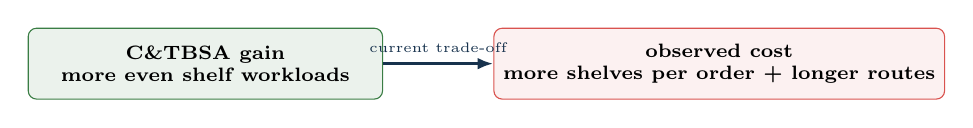
\begin{tikzpicture}[
    box/.style={rounded corners=3pt,minimum width=4.5cm,minimum height=0.9cm,
      align=center,font=\scriptsize\bfseries},
    arr/.style={-{Latex[length=2mm]},very thick,Navy}
  ]
    \node[box,draw=Green,fill=Green!10] (gain) {C\&TBSA gain\\more even shelf workloads};
    \node[box,draw=Red,fill=Red!8,right=14mm of gain] (cost)
      {observed cost\\more shelves per order + longer routes};
    \draw[arr](gain)--node[above,font=\tiny]{current trade-off}(cost);
  \end{tikzpicture}
  \source{Static expected-flow recalculation; the grid has no explicit resource capacities, so raw load is not physical utilization.}
\end{frame}

\begin{frame}{Meeting conclusion: method works, operational trade-off is unresolved}
  \centering
  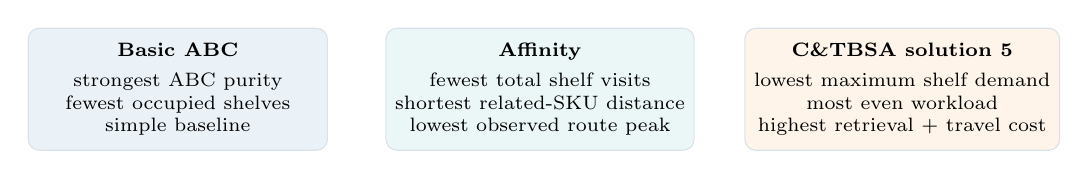
\begin{tikzpicture}[
    card/.style={rounded corners=4pt,minimum width=3.8cm,minimum height=1.55cm,
      align=center,font=\scriptsize,draw=Mid}
  ]
    \node[card,fill=Blue!9] at (0,0)
      {\textbf{Basic ABC}\\[1mm]
       strongest ABC purity\\fewest occupied shelves\\simple baseline};
    \node[card,fill=Cyan!10] at (4.6,0)
      {\textbf{Affinity}\\[1mm]
       fewest total shelf visits\\shortest related-SKU distance\\lowest observed route peak};
    \node[card,fill=Orange!10] at (9.2,0)
      {\textbf{C\&TBSA solution 5}\\[1mm]
       lowest maximum shelf demand\\most even workload\\highest retrieval + travel cost};
  \end{tikzpicture}
  \vspace{0.28cm}
  \begin{alertblock}{Evidence-based interpretation}
    \centering\scriptsize The algorithm reproduction is functioning: its demand-balancing
    objective improved. The current selected Pareto solution does \textbf{not}
    yet provide the desired combined outcome of balanced shelves and low travel.
  \end{alertblock}
  \vspace{0.08cm}
  \begin{block}{Next controlled experiment}
    \centering\scriptsize Compare C\&TBSA solutions 1--5 and seeds 0--2 on this frozen
    input snapshot, then validate the shortlisted trade-off in simulation.
  \end{block}
\end{frame}

\end{document}
